\documentclass[a4paper, 11pt]{article}

% Nécessaire
\usepackage[utf8]{inputenc}
\usepackage[T1]{fontenc}
\usepackage{lmodern}

% Biblio
\usepackage{natbib}
\bibliographystyle{abbrvnat}
\usepackage{hypernat}
\bibpunct{\textcolor{blue}{[}}{\textcolor{blue}{]}}{}{a}{\textcolor{blue}{,}}{;}

\usepackage[french]{babel}
\usepackage{amsmath, amsthm}
\usepackage{amsfonts,amssymb}

% Marge
\usepackage{geometry}
\geometry{margin={2.2cm ,2cm}}

% Figures, graphiques
\usepackage{graphicx}
\usepackage{epsfig}
\usepackage{caption}

% Surlignage
\usepackage{alltt}

\usepackage{xcolor}
\usepackage{soul}
\usepackage{color}
\usepackage{colortbl}

% Indicatrice
\usepackage{dsfont}

\usepackage{multirow}
\usepackage{eurosym}
\usepackage{extarrows}
\usepackage[colorlinks=true, citecolor=blue, linkcolor=.]{hyperref}

% Graphique
\usepackage{tikz}


% Titre
\title{Ajustement de la probabilité de pupaison en fonction de la température}
\author{}
\date{}



\begin{document}
 \maketitle
 
 Jusqu'à présent nous avions dans notre modèle $p_{\text{pup}} = p_p \times \mu_p$ fixé à 0.77. En utilisant une constante, on ne prend pas du tout en compte les conditions externes qui pourrait influencer sur le cycle de développement des cécidomyies (\emph{e.g.} les conditions météorologiques).
 
 Le but est ici d'obtenir une valeur de $p_{\text{pup}}$ qui dépendrait de la température. On choisit la température car cette variable est accesible et qu'elle a, \emph{a minima}, un effet sur la durée de la diapause \citep{a2014}.
 
 \section{La probabilité de pupaison en fonction de la température}
 
  On récupère les données de l'article de \citet{a2014} pour essayer de voir s'il y a un lien entre température et durée de pupaison.
 
 \subsection{Température quotidienne}
 
 On ne considère ici que la température du jour.
 
 \paragraph{Méthode} À chaque date --- pour lesquelles on a des données sur le nombre de larves et le nombre de larves en pupaison --- on calcule la proportion de larves en pupaison. On extrait ensuite les températures moyennes des jours (lissées avec une moyenne mobile d'ordre 3) correspondantes. On effectue ensuite une régression linéaire simple de la proportion de larves en pupaison par la température.
 
 \paragraph{Résultats} La régression linéaire sur nos 14 individus nous donne les résultats visibles dans la table~\ref{tab:lm}. Pour un risque de première espèce fixé à $\alpha = 5\%$, la température est utile à la prédiction de $p_{\text{pup}}$. La figure~\ref{fig:lm} illustre le résultat.
 
 % latex table generated in R 3.5.2 by xtable 1.8-3 package
% Mon Jun 24 12:11:56 2019
\begin{table}[ht]
\centering
\caption{Régression linéaire de la proportion d'individus en pupaison par la température du jour}
\label{tab:lm}
\begin{tabular}{rrrrr}
 & Estimate & Std. Error & t value & Pr($>$$|$t$|$) \\ 
  \hline
(Intercept) & 1.9544 & 0.4014 & 4.87 & 0.0004 \\ 
 temp1j & -0.0549 & 0.0175 & -3.13 & 0.0087 
\end{tabular}
\end{table}
 
\begin{figure}[ht]
\centering
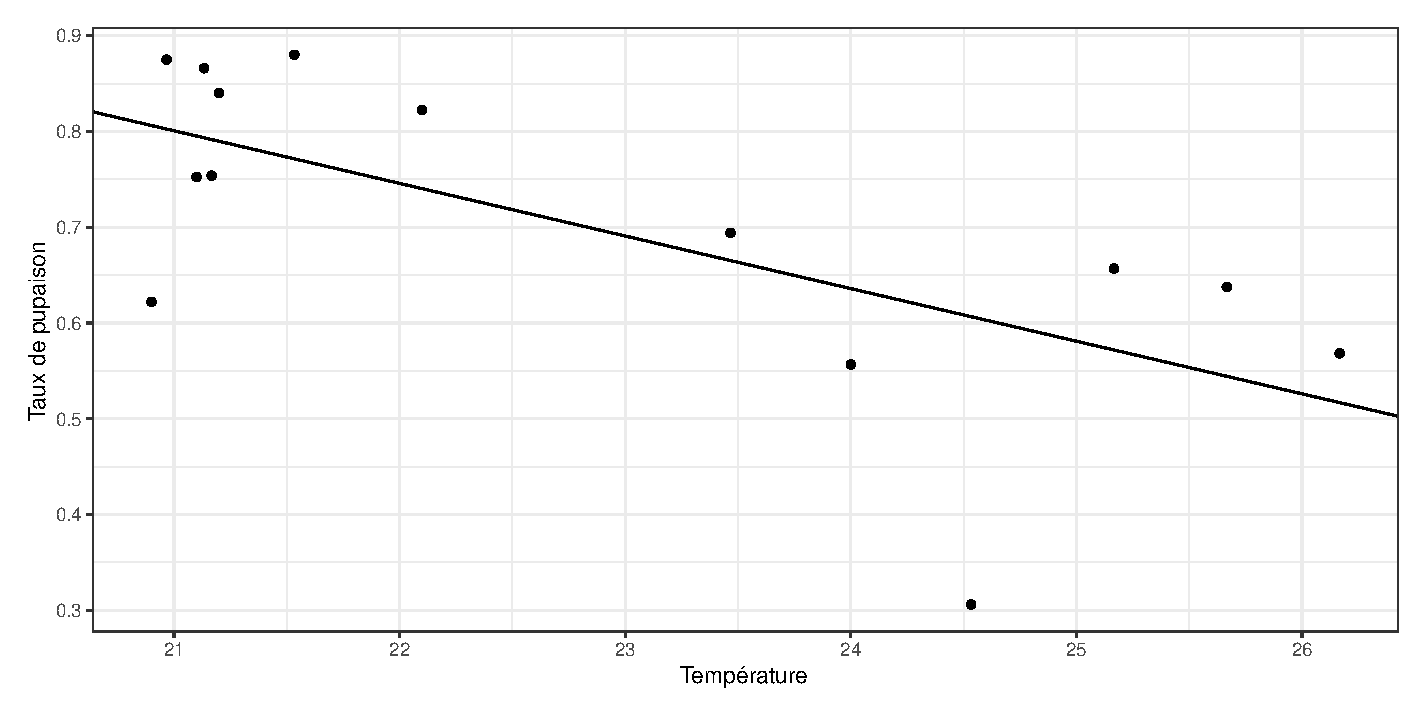
\epsfig{file = plots/lm.eps, scale = 0.65}
 \caption{Droite de la régression linéaire simple.}
 \label{fig:lm}
\end{figure}

\subsection{Température moyenne sur 15 jours}

On réalise ici la même démarche que précédemment sauf que l'on considère la température moyenne sur 15 jours (de 7 jours avant jusqu'à 7 jours après). Les résultats sont visibles dans la table~\ref{tab:lm2}.
Les coefficients de la régression linéaire sont très proches de ceux trouvés précédemment.

% latex table generated in R 3.5.2 by xtable 1.8-3 package
% Fri Jun 28 12:19:43 2019
\begin{table}[hb]
\centering
\caption{Régression linéaire de la proportion d'individus en pupaison par la température moyenne sur 15 jours}
\label{tab:lm2}
\begin{tabular}{rrrrr}
 & Estimate & Std. Error & t value & Pr($>$$|$t$|$) \\ 
  \hline
(Intercept) & 1.9555 & 0.3665 & 5.34 & 0.0002 \\ 
  temp15j & -0.0550 & 0.0160 & -3.43 & 0.0050 \\ 
\end{tabular}
\end{table}

\section{Différences}

La figure~\ref{fig:compup} montre la différence de la probabilité de pupaison à chaque date avec chacune des trois méthodes testées. Sans surprise, la probabilité de pupaison qui est fonction de la température quotidienne fluctue beaucoup. Ce qui est notable, c'est que l'on observe pas une baisse de température en fin de saison. Ce n'est donc pas la température qui explique l'absence de cécidomyies alors qu'il reste des inflorescences.
\begin{figure}[ht]
\centering
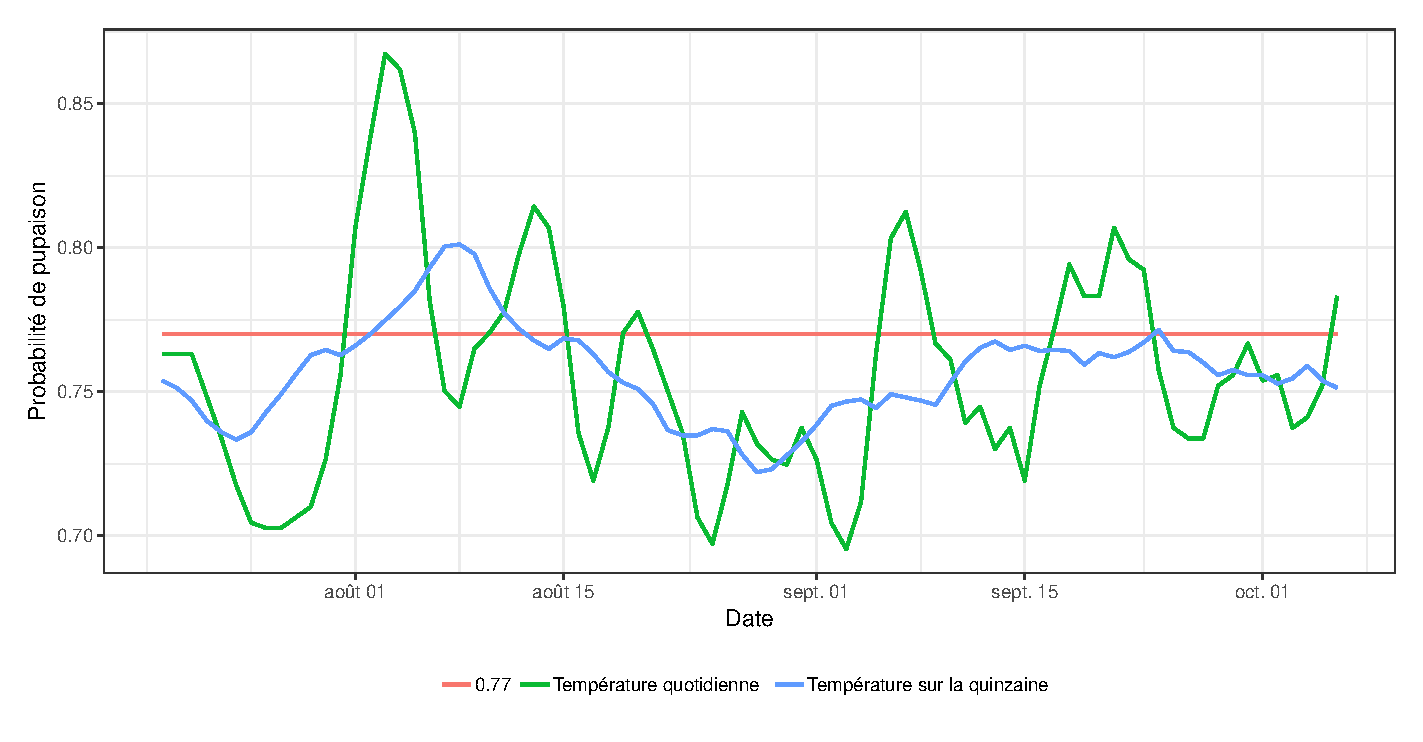
\epsfig{file = plots/comp_ppup.eps, scale = 0.65}
 \caption{Comparaison des différentes probabilités de pupaison}
 \label{fig:compup}
\end{figure}

La figure~\ref{fig:dyn} illustre la différence entre les dynamiques proposées pour un jeu de paramètres fixés
\begin{center}
\begin{tabular}{lllll}
$\gamma$ & $p_m$ & $\mu_{\text{ER}}$ & $\mu_{\text{ER}}$ & $k$\\
0.02 & 0.856 & 1.000 & 1.000 & 54.996
\end{tabular}
\end{center}
Les différences sont négligeables.
\begin{figure}[ht]
\centering
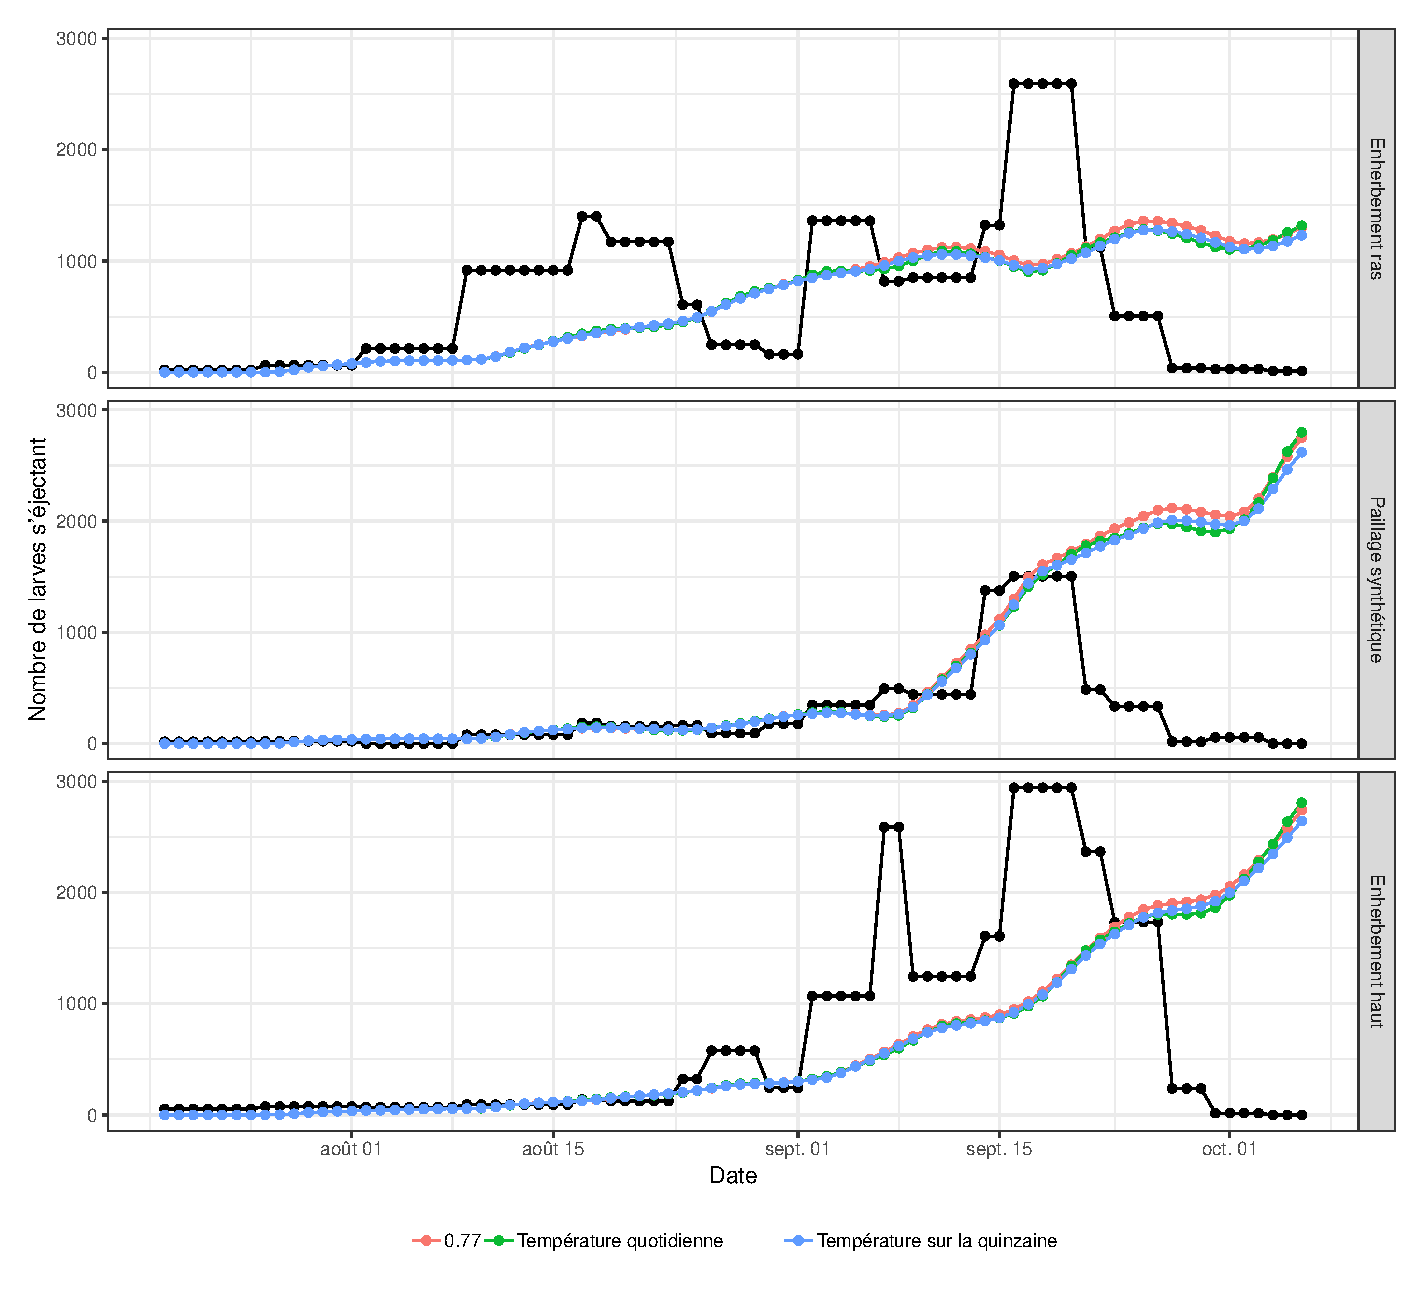
\epsfig{file = plots/comp_dyn_pup.eps, scale = 0.65}
 \caption{Comparaison des différentes dynamiques selon la probabilité de pupaison}
 \label{fig:dyn}
\end{figure}


\clearpage
\bibliography{p_pup}


 \end{document}
 
